\documentclass[10 pt, a4paper]{article}

\usepackage{graphicx}
\usepackage{caption}
\usepackage{anysize}
%\usepackage{changepage}
\usepackage{amsfonts}
\usepackage{float}
\usepackage{todonotes}
\usepackage{amsmath}
\usepackage[toc,page]{appendix}
\usepackage{subcaption}
\usepackage{hyperref}

\marginsize{2 cm}{2 cm}{1 cm}{2 cm}

\captionsetup[figure]{labelfont=bf,textfont=it,width=0.88\textwidth}
\captionsetup[table]{labelfont=bf,textfont=it,width=0.88\textwidth}


\setlength{\parindent}{0 cm}

\title{
  Identifying Hand Written Digits from the MNIST Dataset using Multiple Classifiers \\
  \Large Neural Networks Assignment 1
}

\date{}

\begin{document}

\maketitle

\vspace{-2 cm}

\abstract{There are a lot of classifiers used to classify digits from the MNIST dataset. In this report we achieved an accuracy of 81 \% using a simple distance-based classifier. Used a Bayes Classifier to determine between 2 classes with a accuracy of 93 \% for an easy to distinguish pair and 64 \% for a more difficult pair. Achieved an accuracy of 86 \% using a single layer perceptron. We looked at a gradient descent algorithm and applied it to model a XOR gate. In appendix \ref{sec:mnistgde} we make some observations regarding using this algorithm for the MNIST data. }

\section{Introduction}

The MNIST dataset is one of the more popular datasets used in image processing and machine learning. The MNIST dataset consists of low resolution grey scale images of handwritten digits.  The modified version of this dataset used for this report consist of a training set of 1707 images and a training set of 1000 images (the number of images per digit is shown in table \ref{tab:digits}). Two digits are shown as an example in figure \ref{fig:digits}. These images have a resolution of 16x16 pixels, represented as 256 component vectors with values ranging between -1 and 1. These values were clamped to range from 0 to 1 in preprocessing.

\begin{table}[H] 
\centering
\begin{tabular}{l|ll}
Digit & \# In train set & \# In test set \\ \hline \hline
0     & 319             & 224            \\
1     & 252             & 121            \\
2     & 202             & 101            \\
3     & 131             & 79             \\
4     & 122             & 86             \\
5     & 88              & 55             \\
6     & 151             & 90             \\
7     & 166             & 64             \\
8     & 144             & 92             \\
9     & 132             & 88             \\ \hline
total & 1707            & 1000          
\end{tabular}
\caption{The number of images per digit in the training set and in the test set.}
\label{tab:digits}
\end{table}

There are many algorithms to classify these digits. With classification  is meant identifying to which digit (called the class) an image belongs. These algorithms vary in complexity and accuracy\footnote{Currently the highest accuracy achieved is around 99.79 \%, for example see Romanuke 2016 \cite{mnist}}. In this report we will look at (in order of increasing complexity): a simple distance-based classifier, a Bayes-rule classifier, a single layer perceptron and gradient descent on a network with an hidden layer.

\begin{figure}[H] 
\begin{subfigure}[b]{0.5\textwidth}
\begin{figure}[H]
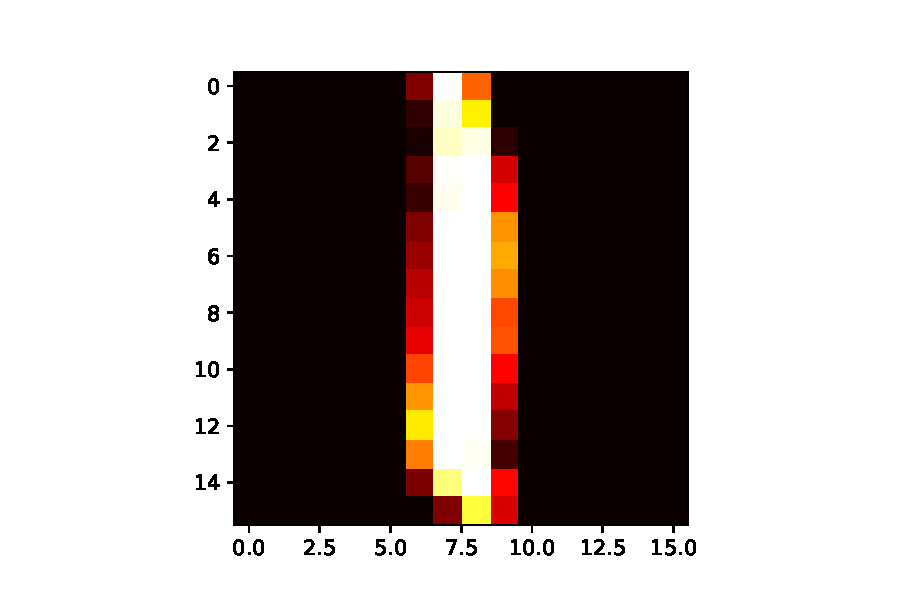
\includegraphics[width=\textwidth]{example_digit_easy}
\caption{One.}
\label{fig:digiteasy}
\end{figure}
\end{subfigure}
\begin{subfigure}[b]{0.5\textwidth}
\begin{figure}[H] 
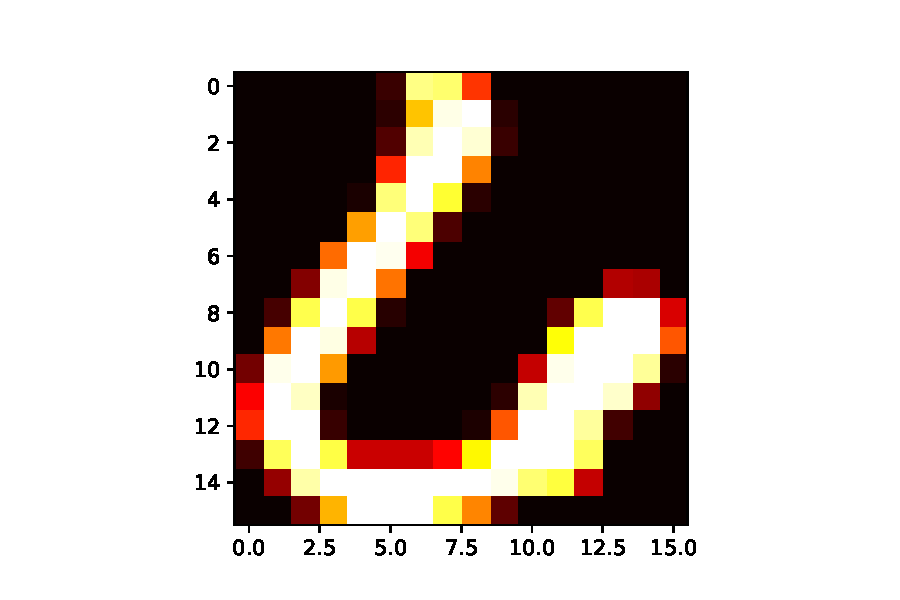
\includegraphics[width=\textwidth]{example_digit_hard}
\caption{Six.}
\label{fig:digithard}
\end{figure}
\end{subfigure}
\caption{Two examples of digits within the dataset. They range from easy to classify (\ref{fig:digiteasy}) to more difficult (\ref{fig:digithard}).}
\label{fig:digits}
\end{figure}

\section{Simple distance-based classifier} \label{sec:dist}

\subsection{Description}

The simple distance-based classifier uses the average vector for all the images belonging to a class within the training set. To classify a image from the test the distance between this vector and the average vectors from the training set are used. The average vector with the smallest distance is the class the image is classified as.
\\
\\
For the distance between the image and the average vectors different metrics can be used. The primary metric used is the euclidean metric given by 

\begin{equation} 
d_{ij} = \sqrt{\sum_n (x^n_i - x^n_j)^2}
\label{eqn:euc}
\end{equation}

where $d_{ij}$ denotes the distance between vector $i$ and $j$, $x^n_i$ denotes the n-th component of the vector $i$ and the sum goes over all dimensions of the vector space (256 in this case). Additional metrics looked at are the Manhattan (or taxicab) metric and the cosine similarity given respectively by

\begin{align}
d_{ij} &= \sum_n \left| x_i^n - x_j^n \right| \label{eqn:man}\\
s_{ij} &= \frac{x_i \cdot x_j}{\sqrt{(x_i)^2} \sqrt{(x_j)^2}} \label{eqn:cos}
\end{align}

where $d_{ij}$ and $x^n_i$ denote the same as in equation \ref{eqn:euc}. $s_{ij}$ is used to denote the cosine similarity between vectors $i$ and $j$ and $(x_i)^2$ is defined as the inner product of the the vector $i$ with itself. 

\subsection{Results}

When the average vectors for each class are calculated the distance between those vectors can be used to predict which classes will be the hardest to distinguish using this classifier. Doing that for the train set using the euclidean metric gives the distance matrix shown in figure \ref{fig:eucdist}. The smaller the distance the more difficult it will be to distinguish them using this classifier. One observation is that 7 \& 9 and 4 \& 9 have a small distance between them and therefore might be difficult to distinguish.

\begin{figure}[H] 
  \centering
    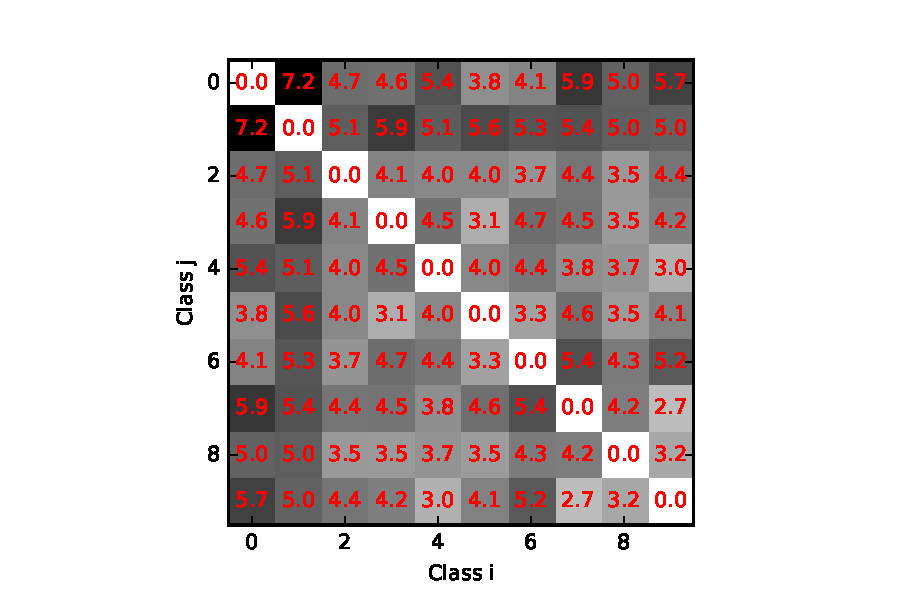
\includegraphics[width=0.7\textwidth]{eucdist}
  \caption{The euclidean distance between the average vectors for each combination of class i and j. The lower the distance the more difficult it will be to distinguish those digits using this distance based classifier. The euclidean metric is symmetric so the distance matrix symmetric. }
  \label{fig:eucdist}
\end{figure}

A different quantity to predict which classes might be difficult to classify is the radius of each class. The radius is defined as the biggest distance between the average vector and the vectors belonging to that class. It gives a metric that indicates how big the difference is in how that digit is written. The radii for each class using the euclidean metric are listed in table \ref{tab:radii}. Most of the radii are similar but the radii of 0 and 1 are relatively big so it might be difficult to classify those images.

\begin{table}[H]
\centering
\begin{tabular}{l|llllllllll}
Class  & 0   & 1   & 2   & 3   & 4   & 5   & 6   & 7   & 8   & 9   \\ \hline
Radius & 7.2 & 7.2 & 5.1 & 5.9 & 5.4 & 5.6 & 5.4 & 5.9 & 5.0 & 5.7
\end{tabular}
\caption{The radius of each of the classes for the training set using the euclidean metric.}
\label{tab:radii}
\end{table}

To verify whether these predictions align with reality the confusion matrix is useful. In this matrix the predicted class is set out against the correct class for the images within the test set. The confusion matrix for the euclidean metric is given in figure \ref{fig:euccom}. Expected was that 7 \& 9 and 4 \& 9 would be difficult to distinguish, in the matrix they indeed have a high confusion number. It was also expected that there would be difficulties with correctly classifying digits belonging to 0 and 1 which the confusion matrix confirms. 

\begin{figure}[H] 
\begin{subfigure}[b]{0.5\textwidth}
\begin{figure}[H]
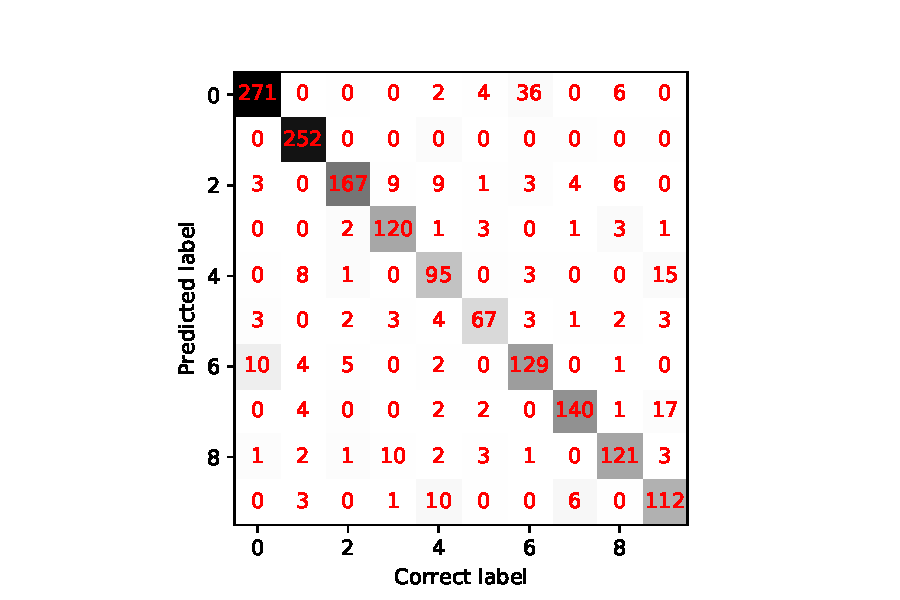
\includegraphics[width=\textwidth]{distanceConfusionTrain}
\caption{Train set.}
\end{figure}
\end{subfigure}
\begin{subfigure}[b]{0.5\textwidth}
\begin{figure}[H] 
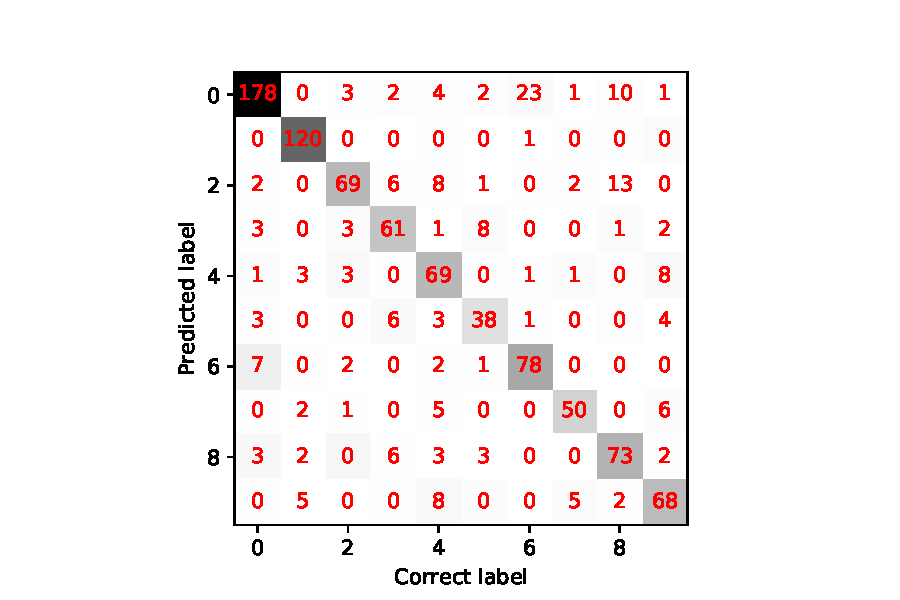
\includegraphics[width=\textwidth]{distanceConfusionTest}
\caption{Test set.}
\end{figure}
\end{subfigure}
\caption{The confusion matrix of the distance based classifier on the train and test set using the euclidean metric.}
\label{fig:euccom}
\end{figure}

To have one number to quantify the performance of a classifier the accuracy is used. The accuracy is defined as the percentage of images within a set that was classified correctly. For the simple distance based classifier using the euclidean metric an accuracy of 85 \% was achieved for the training set and 79 \% for the test set.
\\
\\
When the Manhattan metric as given by equation \ref{eqn:man} is used an accuracy of 77 \% was achieved on the train set and 72 \% on the test set. This is worse than the euclidean metric. For the euclidean metric the shortest distance between 2 points is uniquely defined but for the Manhattan metric this is not the case, there might be multiple paths between two points with the same distance. This might explain why the simple distance-based classifier achieves an lower accuracy using the Manhattan metric.
\\
\\
When the cosine similarity as given by equation \ref{eqn:cos} is used to define the distance between vectors an accuracy of 87 \% is achieved on the training set and 81 \% on the test set. This is better than the euclidean metric. The main advantage of using the cosine similarity as a metric is that it ignores the norm of the vector and only looks at the direction. For our data the norm is relevant so why it performs better than the euclidean metric for this data is not understood.



\section{Bayes-Rule classifier}

\subsection{Description}

A different strategy to classify the digits is to look at a specific feature within the dataset, for example the height-width ratio of the images. To simplify things somewhat we only look at two classes within the dataset. To train the classifier look at the height-width ratio of the images belonging to one of the two classes within the training set. Then construct a histogram of the distribution of the height-width ratio and use Bayes rule to determine the chance a new image belongs to digit $a$ or $b$ given the height-width ratio of this image from the test set. Bayes rule is given by

\begin{equation}
P(C_k | X) = \frac{P(X|C_k)P(C_k)}{P(X)}
\label{eqn:bayes}
\end{equation} 

where $P(C_k | X)$ is the chance that the correct classification is $C_k$ given an image $X$ (called the posterior), $P(X | C_k)$ is the chance that an image $X$ is classified as $C_k$ (called the class-conditional), $P(C_k)$ is the overall chance that an image belongs to class $C_k$ (called the prior) and $P(X)$ is the scaling factor which is equal to $1$ in this case.

\subsection{Results}

For these results we look at two pairs of classes within our dataset. We look at a pair where the height-width ratio is expected to be similar and at a pair where it is expected to be further apart, 5 \& 7 and 1 \& 4 respectively. From table \ref{tab:digits} we can see that the training set contains 88 fives, 166 sevens, 252 ones and 122 fours. To see how the height-width ratio is distributed for both of these pairs we plot a histogram (see figure \ref{fig:hist}). Here we can see that within these pairs the difference between the height width ratio is different as expected.

\begin{figure}[H] 
\begin{subfigure}[b]{0.5\textwidth}
\begin{figure}[H]
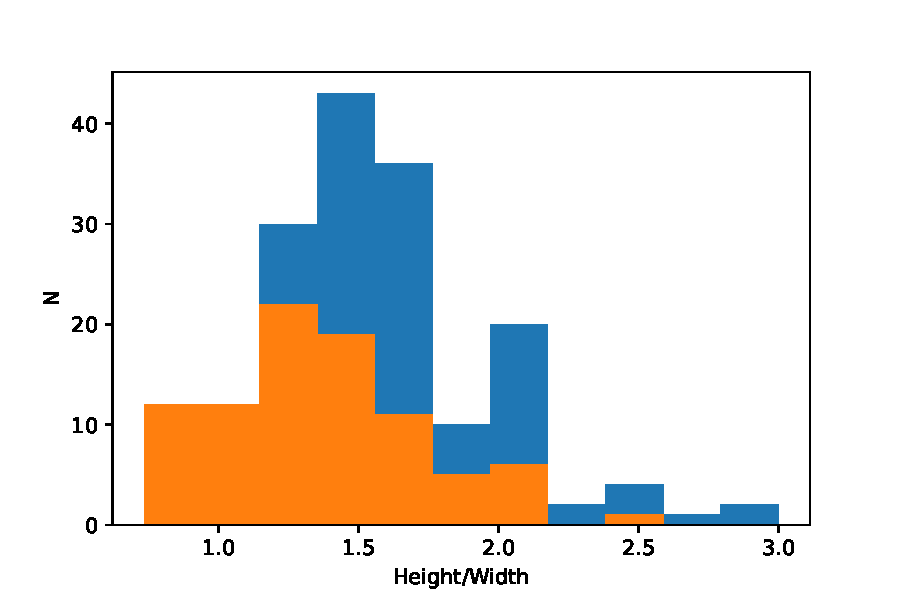
\includegraphics[width=\textwidth]{hist57}
\caption{Blue: seven, orange: five.}
\label{}
\end{figure}
\end{subfigure}
\begin{subfigure}[b]{0.5\textwidth}
\begin{figure}[H] 
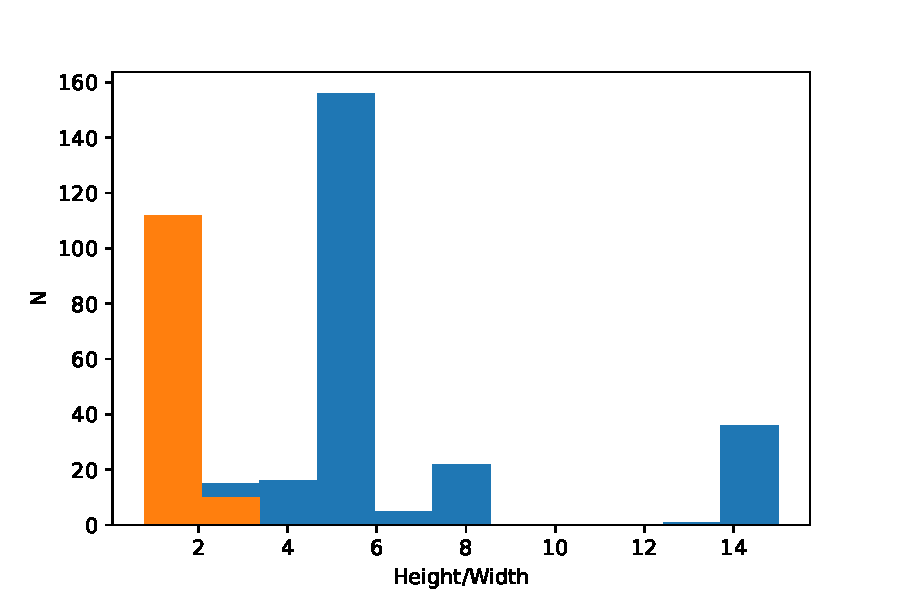
\includegraphics[width=\textwidth]{hist14}
\caption{Blue: one, orange: four.}
\label{}
\end{figure}
\end{subfigure}
\caption{Histograms for both of the pairs of classes we look at. The height of the bars represent how many images within the training set are in the bins in the height-width ratio.}
\label{fig:hist}
\end{figure}

Than we can calculate $P(X|C)$ and $P(C)$ from this histogram for both of the pairs separately. We than use equation \ref{eqn:bayes} to calculate $P(C|X)$. We than use this result to classify the pairs within our test dataset.
\\
\\
Using this method an accuracy of  63 \% was achieved on the training set and 64 \% on the test set for the 5 \& 7 pair. For the 1 \& 4 pair an accuracy of 96 \% was achieved on the training set and 93 \% on the test set. For one pair the accuracy is higher on the test set than on the train set. This might indicate that in the test set the images belonging to that particular class might have been grouped closely together than was the case in the train set.


\section{Single-Layer perceptron} \label{sec:perceptron}

\subsection{Description}

The single-layer perceptron was among the first algorithms for neural networks proposed by Rosenblatt in 1958 \cite{rosenblatt}. It uses a set of weights and a biases to make a prediction to which of the 10 classes the image from the train set belongs. This prediction is then compared with the known correct answer. If the prediction was correct the weights remain the same, if the prediction was incorrect the weights are nudged in the direction of the correct answer and nudged in the opposite direction of the (incorrect) prediction. This is done for each image in the training dataset multiple times until the predictions stop improving (or our weights correctly predict all the images in the training set).
\\
\\
To look at the process quantitatively look at the number of misclassification's per loop over all the images within the training set. This will give a metric to study the speed with which the perceptron converges towards a set of weights. This than gives  a metric to compare different strategies for initialization of the weights. 

\subsection{Results}

When we apply the single-layer perceptron algorithm to the training set it usually reaches perfect classification at about 45 iterations. The exact amount of iterations varies because of the random initial weights. When these weights are used to classify the images from the test set a accuracy of about 86 \% is achieved, the exact accuracy also varies because of the random initial weights. For the train set a accuracy of 100 \% is achieved so at some point the perceptron has 'memorized' all of  the images and will stop improving.

\begin{figure}
  \centering
    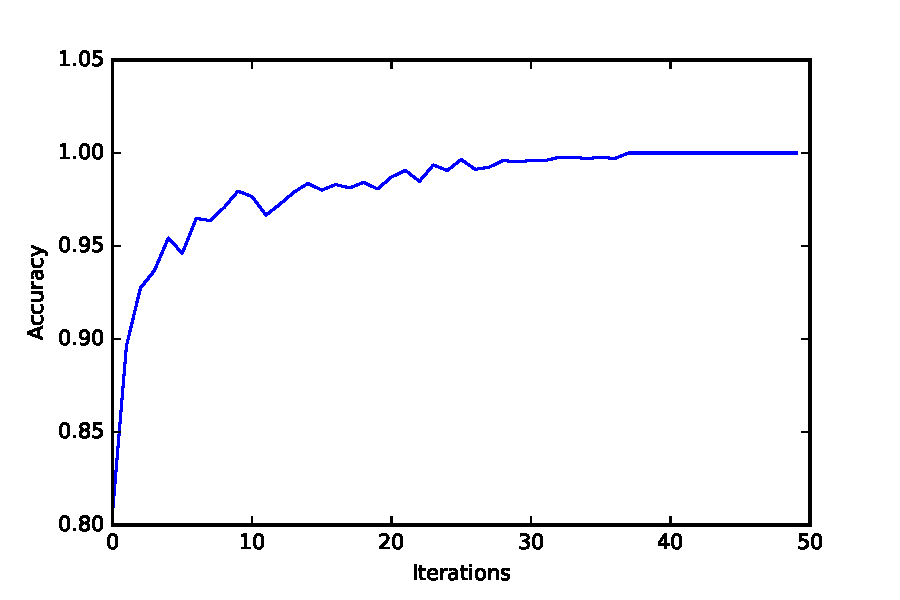
\includegraphics[width=0.7\textwidth]{perceptron_accuracy}
  \caption{Diagram depicting how the accuracy increases during the training of the perceptron algorithm. one can see that after $\pm 40$ iterations the perceptron achieves perfect classification of the training dataset. }
  \label{fig:percom}
\end{figure}

The confusion matrix for the perceptron (figure \ref{fig:percom}) looks similar to the confusion matrix for the distance based classifier (figure \ref{fig:euccom}). Both of the classifiers have difficulties classifying the zeros and ones.

\begin{figure}[H] 
  \centering
    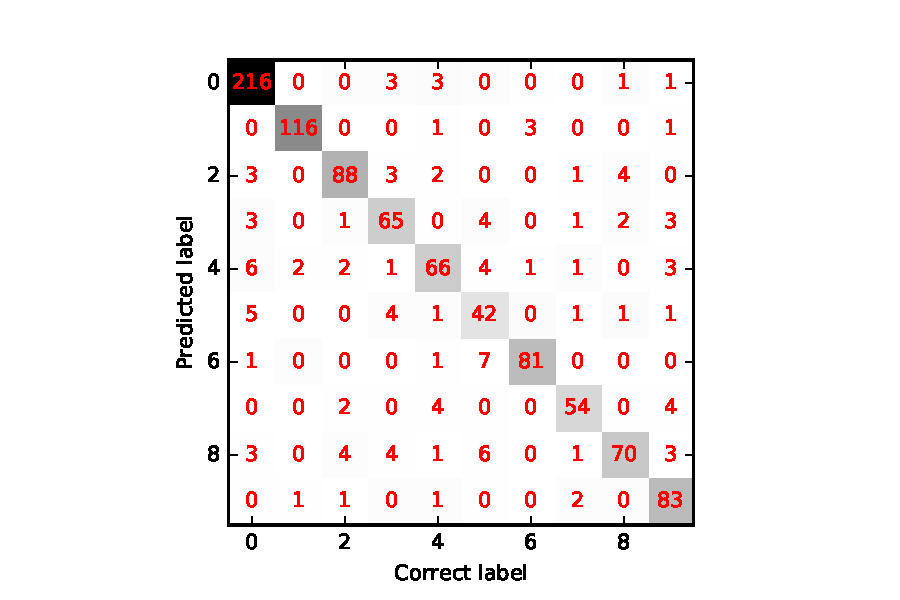
\includegraphics[width=0.7\textwidth]{perceptronConfusion}
  \caption{The confusion matrix for the single layer perceptron on the test set. }
  \label{fig:euccom}
\end{figure}

\section{Gradient descent} \label{sec:gde}

\subsection{Description}

The single-layer perceptron algorithm used in section \ref{sec:perceptron} takes a rather blunt approach to updating the weights. A more refined approach can be taken by looking at the network as a multivariate function. Then a cost function can be defined and that function minimized. The cost function used in this algorithm called the mean squared average is given by

\begin{align}
\mathrm{MSE} = \frac{1}{N} \Sigma_i (X_i - \hat{X}_i)^2
\end{align}

where $X_i$ are the images within the train set and $\hat{X}_i$ the correct label for that images. The factor $1/N$ is for normalization.
\\
\\
Now finding the optimal set of weighs can be seen as finding a minimum of this cost function. To calculate the direction towards a minimum the gradient of the function is used. The gradient gives a vector in the direction of strongest ascent. So when we nudge our weights in the opposite direction we will take the fastest route towards a minimum of the cost function. To control how fast the minimum is approached a parameter called the learning rate $\eta$ is introduced. The gradient vector is multiplied with $\eta$ to control the speed. The higher the value of $\eta$ the faster the minimum is approached but higher the chance of skipping over a minimum. The weights are initialized randomly between -1 and 1. Initialization at zero would result a gradient equal to the zero vector and therefore would not work.
\\
\\
The minimum that the model reaches isn't guaranteed to be a global minimum. It is likely that it is a local minimum and this means that the weights that this algorithm find aren't guaranteed to be the optimal set of weights. To get around this the algorithm could be run multiple times and look which minimum gives the best accuracy.
\\
\\
To get a feel for this algorithm we apply it to model a XOR gate which corresponds with the following truth table:

\begin{table}[H]
\centering
\begin{tabular}{ll|l}
x & y & z \\ \hline
0 & 0 & 0 \\
0 & 1 & 1 \\
1 & 0 & 1 \\
1 & 1 & 0
\end{tabular}
\caption{Given inputs $x,y$ the output $z$.}
\end{table}

We look at a network with 2 input nodes corresponding with inputs $x$ and $y$, a hidden layer with 2 nodes and 1 output node corresponding with the output $z$. Both the input layer and the hidden layer have an extra node to function as a bias node. At each of the nodes in the hidden layer and in the output layer we apply an activation function to the inputs of the nodes.
\\
\\
For this activation function there are multiple options. In this report we look at the sigmoid function, linear rectifier and the hyperbolic tangent respectively given by

\begin{align}
\sigma (x) &= \frac{1}{1 + e^{-x}} \\
R (x) &= \mathrm{max}(0,x) \\
\tanh (x) &= \frac{2}{1 + e^{-2x}} - 1.
\end{align}

\subsection{Results}

When we train our network for the XOR gate we can observe how the mean squared error varies over time. Due to this random initialization the algorithm does not always reach the same minimum mean squared error. In figure \ref{fig:xormsenice} we can see a run where the mean squared error approaches zero and the achieved accuracy is 100 \%. In figure \ref{fig:xormsefail} we can see a run where the mean squared error converges to $\sim 0.13$ and the accuracy is only 50 \% which is as good as a random guess. 

\begin{figure}[H] 
\begin{subfigure}[b]{0.5\textwidth}
  \centering
    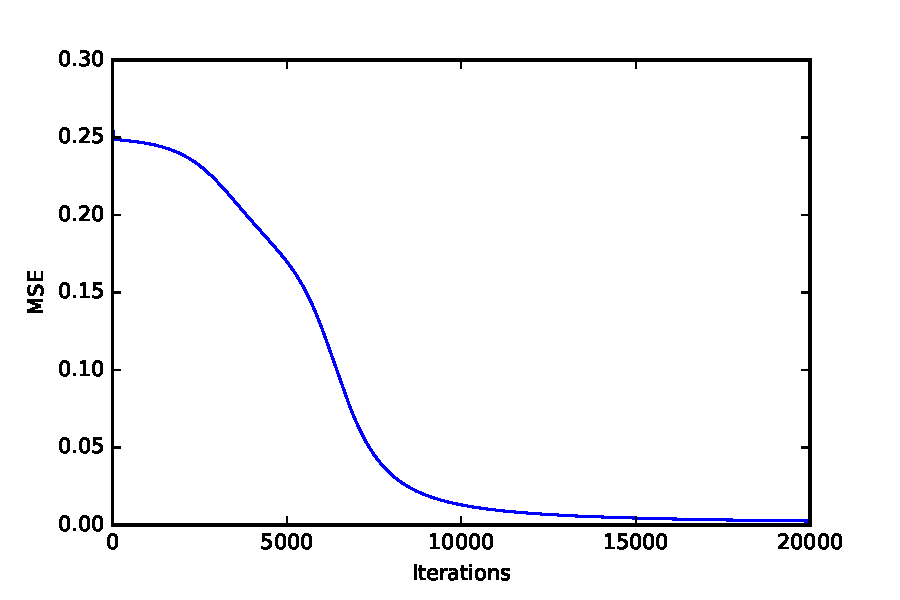
\includegraphics[width=\textwidth]{xor_mse}
  \caption{Mean squared error}
\end{subfigure}
\begin{subfigure}[b]{0.5\textwidth} 
  \centering
    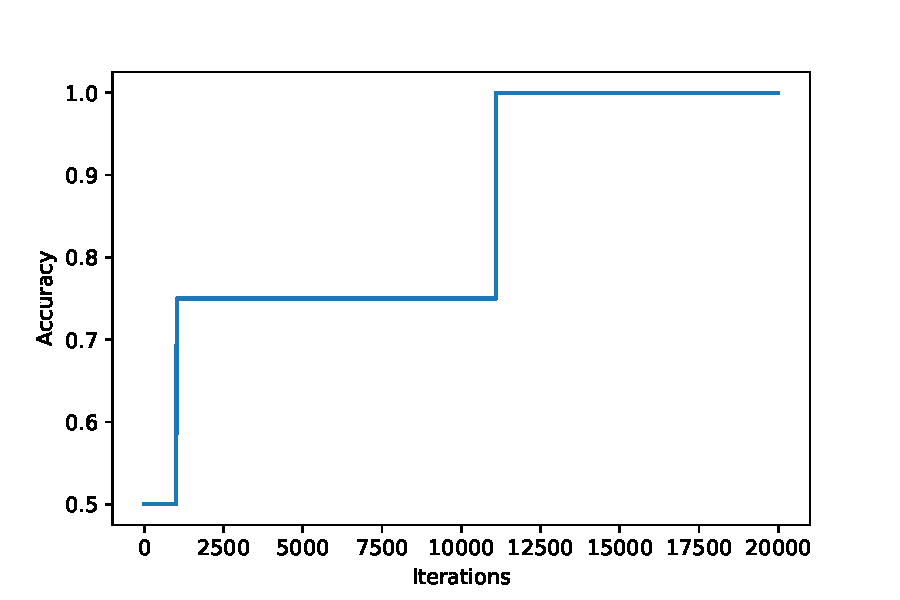
\includegraphics[width=\textwidth]{xor_acc}
  \caption{Accuracy}
\end{subfigure}
\caption{The mean squared error and accuracy for the gradient descent algorithm for the XOR data with $\eta = 0.1$ where the sigmoid function was used as the activation function. In this run the network converges to an accuracy of 1 and an mean squared error of 0.}
  \label{fig:xormsenice}
\end{figure}

\begin{figure}[H] 
\begin{subfigure}[b]{0.5\textwidth}
  \centering
    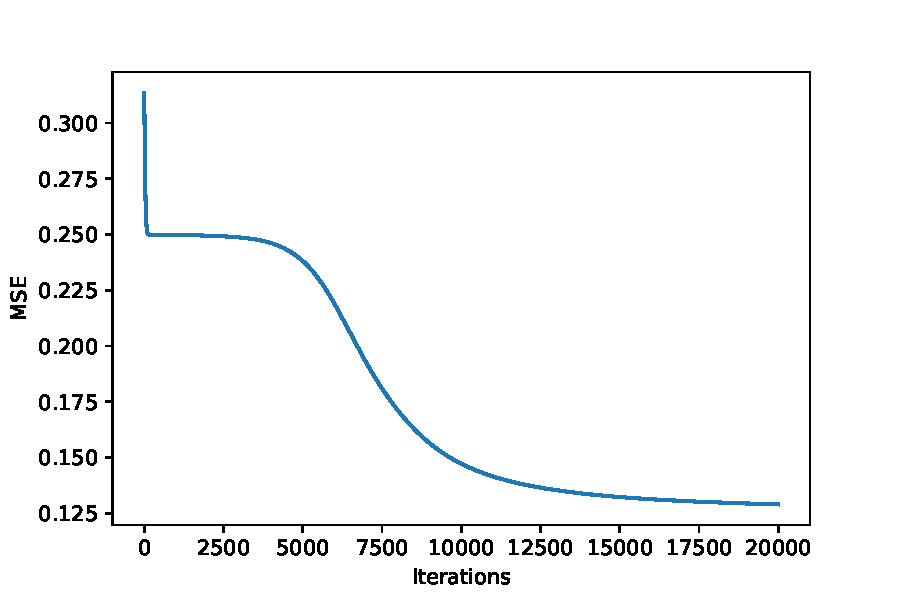
\includegraphics[width=\textwidth]{xor_mse_fail}
  \caption{Mean squared error}
\end{subfigure}
\begin{subfigure}[b]{0.5\textwidth} 
  \centering
    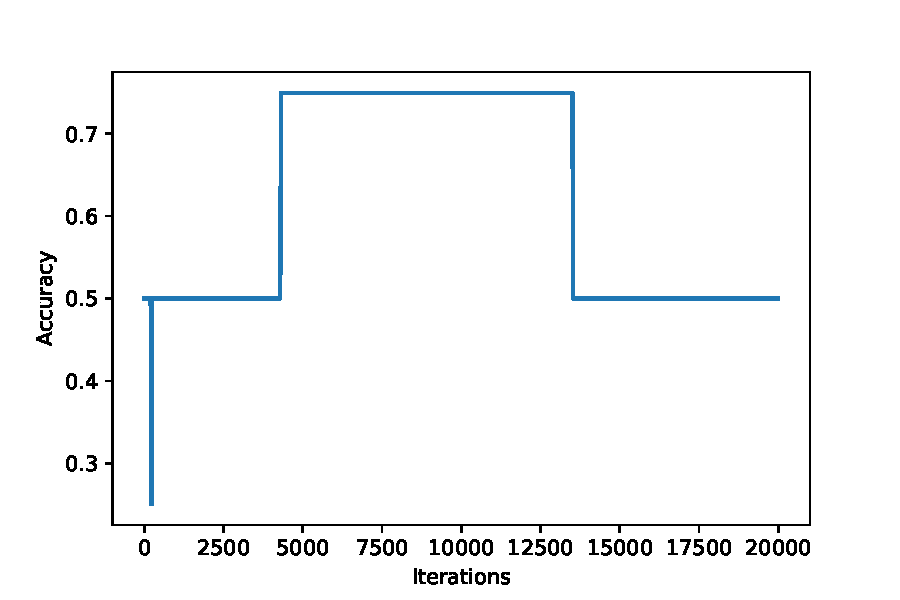
\includegraphics[width=\textwidth]{xor_acc_fail}
  \caption{Accuracy}
\end{subfigure}
\caption{The mean squared error and accuracy for the gradient descent algorithm for the XOR data with $\eta = 0.1$ where the sigmoid function was used as the activation function. In this run the network converges to an accuracy of 0.5 and an mean squared error of $\sim 0.13\%$.}
  \label{fig:xormsefail}
\end{figure}

We can also look at varying $\eta$, when we decrease $\eta$ it will converge slower towards a minimum and the chance is bigger it gets stuck in a small local minimum. When we increase $\eta$ it will converge faster towards a minimum but the chance will get bigger we 'skip' over the minimum. Since our network converges towards a minimum where the mean squared error is zero the improvement a different $\eta$ could give is a shorter runtime (less iterations). Therefore we look at a bigger value for $\eta$ than $\eta = 0.1$ that we used for figure \ref{fig:xormsenice} and \ref{fig:xormsefail}. When we run the model for bigger $\eta$ we indeed notice that the amount of iterations needed before we reach a minimum indeed decreases, the trade off is that there are more runs where the minimum that the model converges to a minimum other than mean a squared error of zero. For example when $\eta = 1.5$ the model converges in about 1000 iterations, which is a factor 20 smaller than for $\eta = 0.1$. When we look at even bigger values of $\eta$ the convergence gets noisy (see figure \ref{fig:xormsenoise})

\begin{figure}[H] 
\begin{subfigure}[b]{0.5\textwidth}
  \centering
    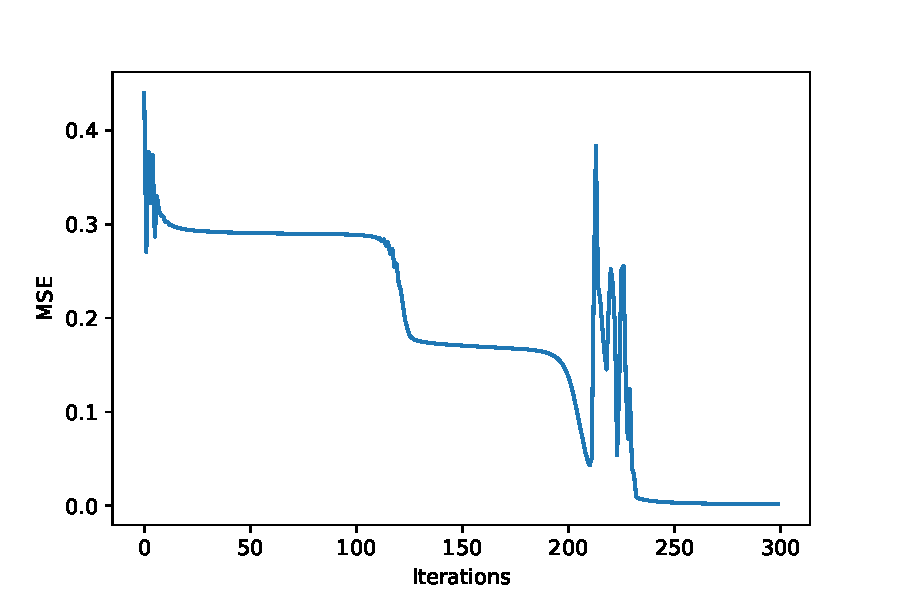
\includegraphics[width=\textwidth]{xor_mse_noise}
  \caption{Mean squared error}
\end{subfigure}
\begin{subfigure}[b]{0.5\textwidth} 
  \centering
    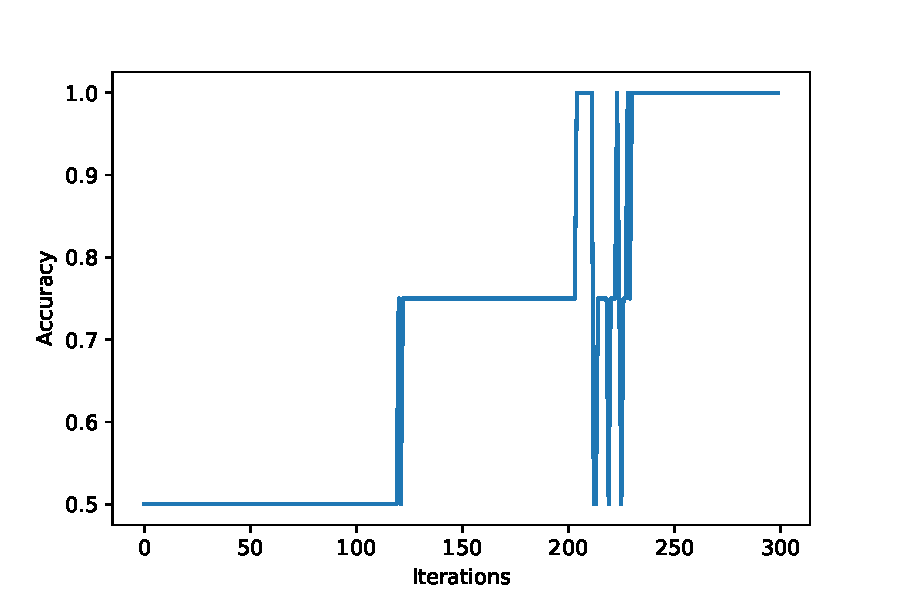
\includegraphics[width=\textwidth]{xor_acc_noise}
  \caption{Accuracy}
\end{subfigure}
\caption{The mean squared error and accuracy for the gradient descent algorithm for the XOR data with $\eta = 20$ where the sigmoid function was used as the activation function. In this run the network converges to an accuracy of 1 and an mean squared error of 0. Visible is that there is some noise in the convergence where we skip over some minima due to the high value of $\eta$.}
  \label{fig:xormsenoise}
\end{figure}


When we look at the three different activation functions as given in \ref{sec:gde} we get different model behaviours given in figure \ref{fig:xormseact}. We see that the sigmoid function is slower to converge than the other two functions for this run. This is consistent with observations over multiple runs. The other two functions did converge faster but also seemed to converge a suboptimal minimum more often. The linear rectifier seemed more noisy, this might be due to the discontinuity this function has at $x = 0$. 

\begin{figure}[H] 
\begin{subfigure}[b]{0.33\textwidth}
  \centering
    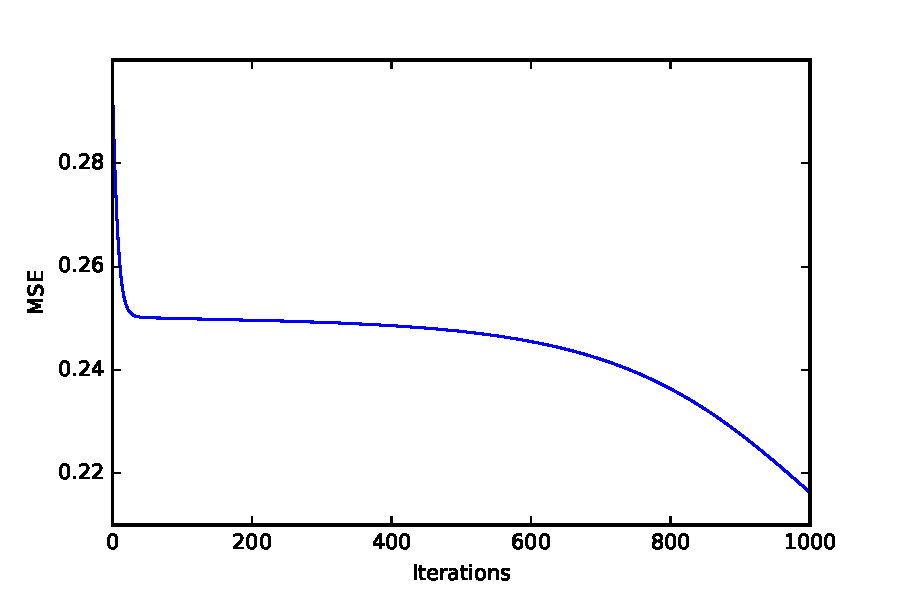
\includegraphics[width=\textwidth]{xor_mse_sig}
  \caption{Sigmoid function.}
\end{subfigure}
\begin{subfigure}[b]{0.33\textwidth} 
  \centering
    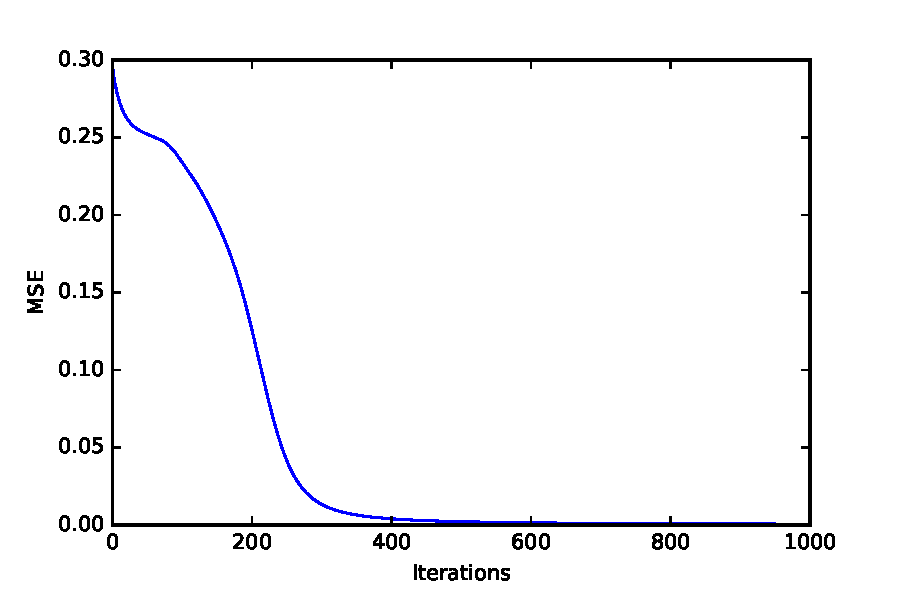
\includegraphics[width=\textwidth]{xor_mse_tanh}
  \caption{Hyperbolic Tangent function.}
\end{subfigure}
\begin{subfigure}[b]{0.33\textwidth} 
  \centering
    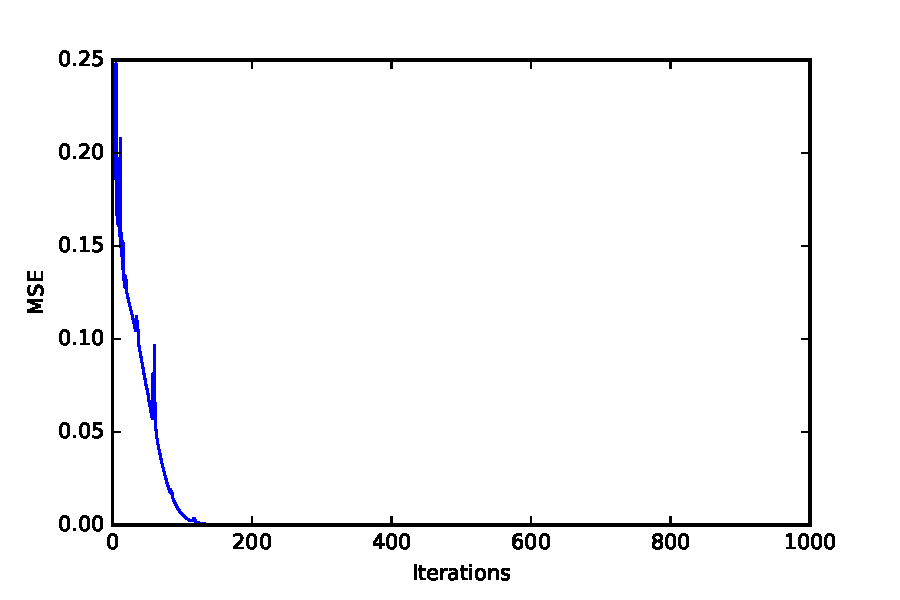
\includegraphics[width=\textwidth]{xor_mse_relu}
  \caption{Linear Rectifier.}
\end{subfigure}
\caption{The mean squared error for the gradient descent algorithm for the XOR data with $\eta = 0.5$. Three different activation functions are used. Visible is that for the different activation functions there is different behaviour for the network.}
  \label{fig:xormseact}
\end{figure}


\section{Discussion \& Conclusion}

We looked at multiple simple algorithms to classify a dataset. When we look at the the simple distance based classifier we see the maximal accuracy we achieved (using cosine similarity) was 81 \% on the test set.
\\
\\
The Bayes classifier reached the highest accuracy of all of the classifiers used but only for 1 pair of digits, for the rest it is the lowest. This algorithm could be expanded to function as a multi class classifier but that would make it more complex and decrease the accuracy.
\\
\\
For the perceptron we achieve 86 \% accuracy on the test set. The accuracy on the train set it reaches 100 \%. This could be an indication that the network 'remembered' all of the images in the training set which could mean that the accuracy on the test set might increase if we feed the model more training data. 
\\
\\
The gradient descent algorithm was only applied on the XOR model so it can not be easily compared to the other classifiers used.


\begin{thebibliography}{99}
\bibitem{rosenblatt} F. Rossenblatt 1958, \textit{The perceptron: A probabilistic model for information storage and organization in the brain}, Psychological Review, Vol 65(6), Nov 1958, 386-408.

\bibitem{neural} M. Nielsen 2019, \textit{Neural networks and Deep Learning}, Chapter 2, \url{http://neuralnetworksanddeeplearning.com/chap2.html}, retrieved on 11-03-2019.

\bibitem{mnist} V. Romanuke 2016, \textit{Training data expansion and boosting of convolutional neural networks for reducing the MNIST dataset error rate},  Research Bulletin of NTUU “Kyiv Polytechnic Institute”, Vol 6, 29–34. 

\end{thebibliography}

\begin{appendices}
\section{Gradient descent for the reduced MNIST dataset} \label{sec:mnistgde}

The code written for section \ref{sec:gde} was changed in order to work for the reduced MNIST dataset used in section \ref{sec:dist} through \ref{sec:perceptron}. To attempt to classify the images a network with 256 input nodes, a hidden layer with 30 nodes and an output layer with 10 nodes was used. The input layer and the hidden layer have an added node to function as a bias node. The simple gradient descent algorithm used for \ref{sec:gde} is inefficient, it is fast enough to converge for the XOR dataset with only 2 inputs and 1 output but for the MNIST case it is not fast enough. In the algorithm used in section \ref{sec:gde} we take the mean squared average error over the entire dataset and use that to update our weights. For the XOR data with only 4 data points this does not give problems but for our MNIST data with 1707 images in the training set this is very inefficient. Changes that could be made are updating the weights after every data point (stochastic gradient descent \cite{neural}) or updating the weights after smaller batches of data (mini batch gradient descent \cite{neural}). Attempts were made but due to time constraints the required changes to the algorithm could not be made in time to get satisfactory results for the MNIST data.

\end{appendices}

\end{document}